\section{Deployment}

\subsection{Architecture}
\begin{itemize}
  \item Server HTTP framework: Flask
  \item Deployed platform: Docker
\end{itemize}


\subsection{Resources}

\begin{itemize}
  \item Deploy from: \url{https://github.com/ai-dave/capstone/tree/main/deploy} 
  \item Deployed model: \url{http://45.33.108.171/home}
\end{itemize}


\begin{figure}
  \centering
  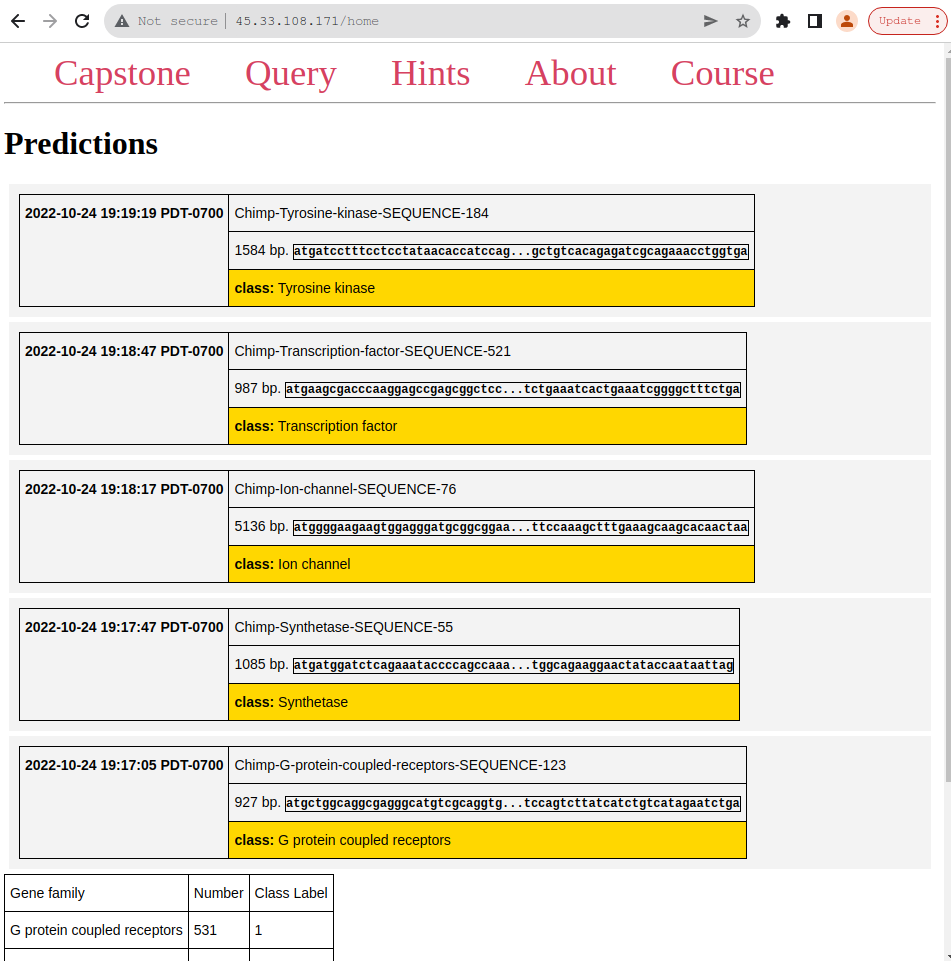
\includegraphics[scale=0.4]{capstone-home}
  \caption{%
     Home landing page showing prediction results for queries submitted.
  }
  \label{fig:capstone-home}
\end{figure}
%

\begin{figure}
  \centering
  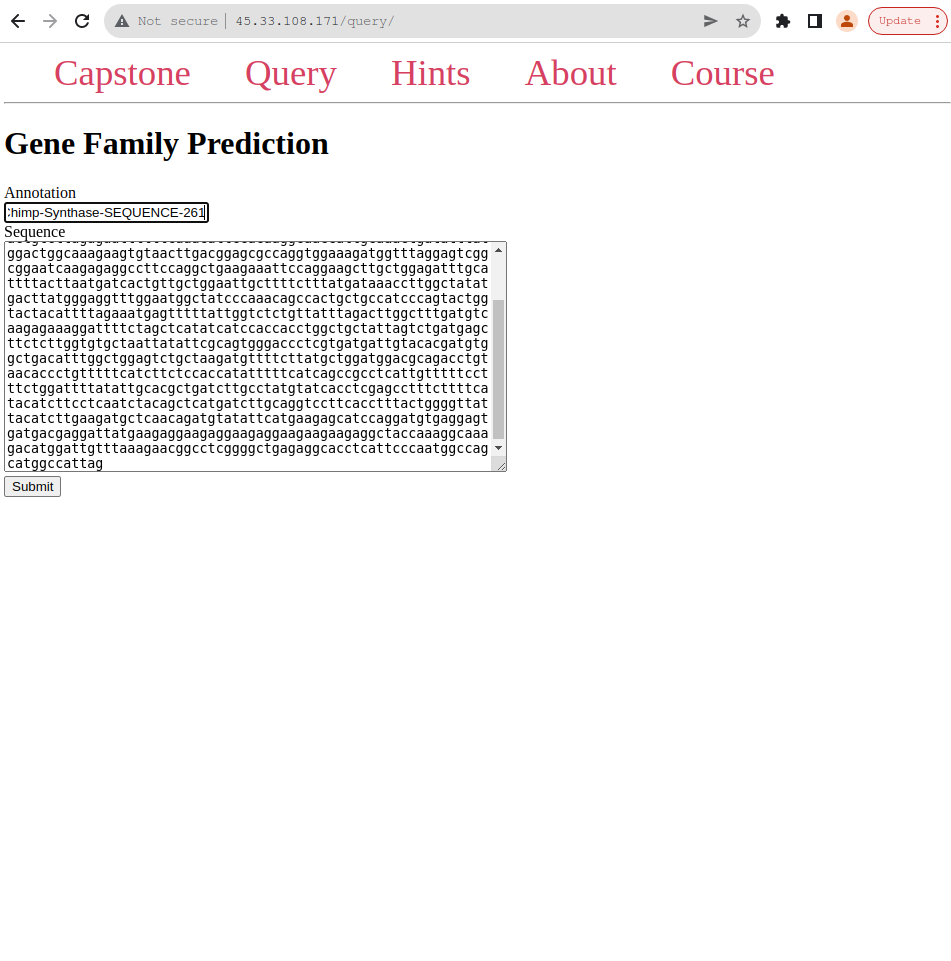
\includegraphics[scale=0.4]{capstone-query}
  \caption{%
     Query form for submitting requests.
  }
  \label{fig:capstone-query}
\end{figure}
%

\begin{figure}
  \centering
  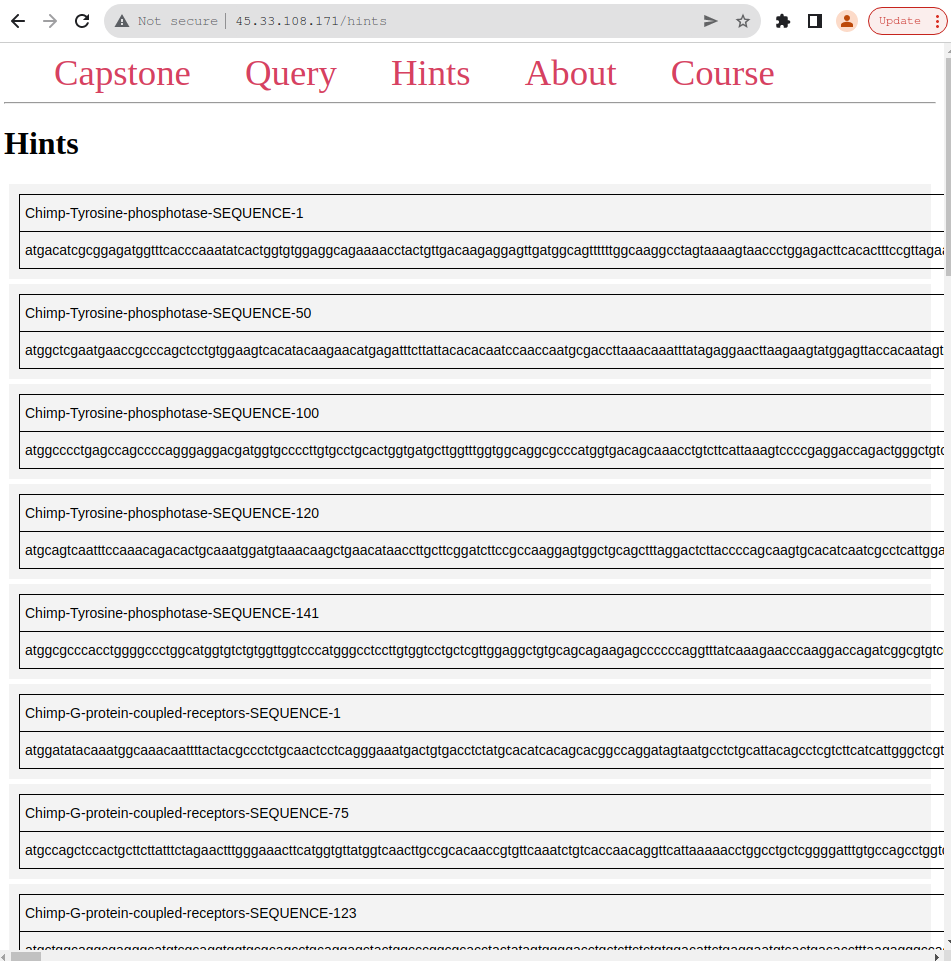
\includegraphics[scale=0.4]{capstone-hints}
  \caption{%
     Sample DNA Coding Sequences with Annotations that can be used for querying.
  }
  \label{fig:capstone-hints}
\end{figure}
%


\begin{figure}
  \centering
  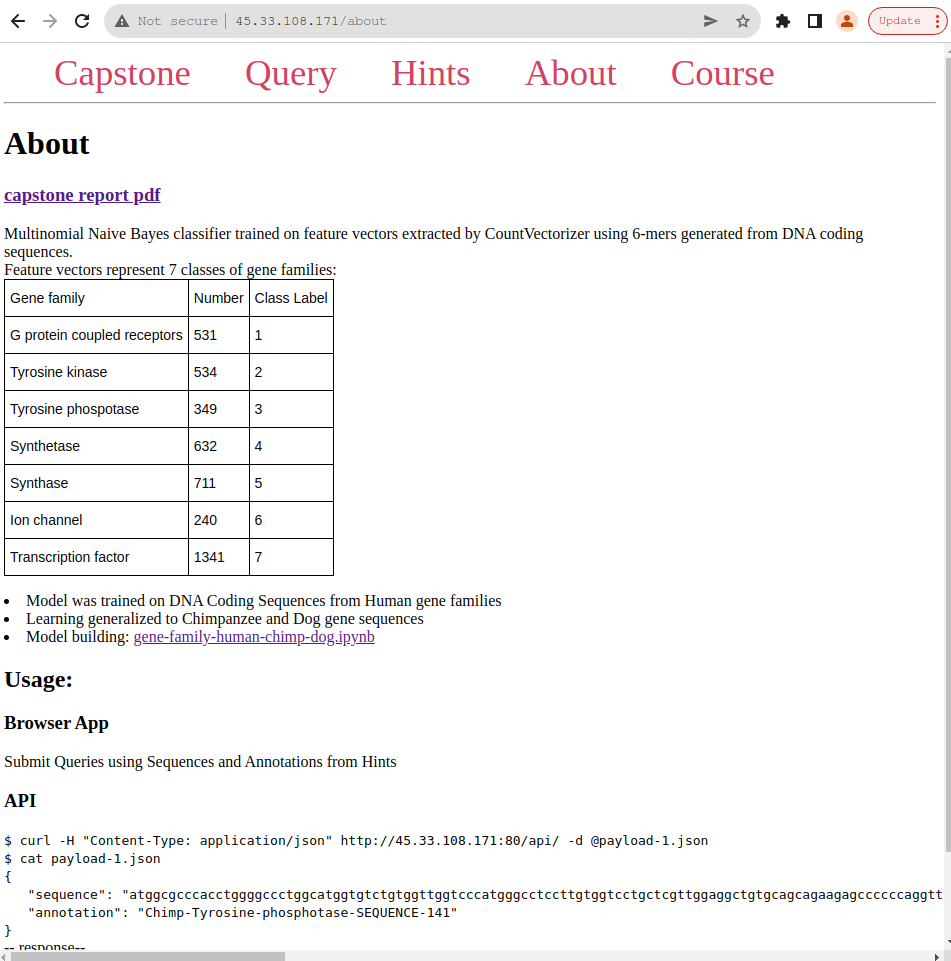
\includegraphics[scale=0.4]{capstone-about}
  \caption{%
     Brief description of the application.
  }
  \label{fig:capstone-about}
\end{figure}
%